% Topic T1.3: FinTech vs. Crypto/DeFi
% Self-contained Beamer slides for Digital Finance course
\documentclass[11pt,aspectratio=169]{beamer}
\usetheme{Madrid}

% ======================= PACKAGES =======================
\usepackage{graphicx}
\usepackage{booktabs}
\usepackage{adjustbox}
\usepackage{multicol}
\usepackage{amsmath}
\usepackage{amssymb}
\usepackage{tikz}
\usetikzlibrary{arrows,shapes,positioning,shadows,trees}
\usepackage{listings}
\usepackage{xcolor}

% ======================= COLOR DEFINITIONS =======================
% Primary color scheme: Blue/Teal for Digital Finance
\definecolor{dfblue}{RGB}{0,102,204}
\definecolor{dfteal}{RGB}{0,153,153}
\definecolor{dfcyan}{RGB}{51,187,204}
\definecolor{dflightblue}{RGB}{153,204,255}
\definecolor{dflightblue2}{RGB}{173,214,255}
\definecolor{dflightblue3}{RGB}{193,224,255}
\definecolor{dflightblue4}{RGB}{213,234,255}

% Accent colors for finance applications
\definecolor{dfgreen}{RGB}{44, 160, 44}
\definecolor{dfred}{RGB}{214, 39, 40}
\definecolor{dforange}{RGB}{255, 127, 14}
\definecolor{dfgray}{RGB}{127, 127, 127}

% Utility colors
\definecolor{lightgray}{RGB}{240, 240, 240}
\definecolor{midgray}{RGB}{180, 180, 180}
\definecolor{codebg}{RGB}{245, 245, 245}

% ======================= THEME CUSTOMIZATION =======================
% Apply Digital Finance color scheme to Madrid theme
\setbeamercolor{palette primary}{bg=dflightblue3,fg=dfblue}
\setbeamercolor{palette secondary}{bg=dflightblue2,fg=dfblue}
\setbeamercolor{palette tertiary}{bg=dfteal,fg=white}
\setbeamercolor{palette quaternary}{bg=dfblue,fg=white}

\setbeamercolor{structure}{fg=dfblue}
\setbeamercolor{section in toc}{fg=dfblue}
\setbeamercolor{subsection in toc}{fg=dfteal}
\setbeamercolor{title}{fg=dfblue}
\setbeamercolor{frametitle}{fg=dfblue,bg=dflightblue3}
\setbeamercolor{block title}{bg=dflightblue2,fg=dfblue}
\setbeamercolor{block body}{bg=dflightblue4,fg=black}

% Remove navigation symbols for cleaner look
\setbeamertemplate{navigation symbols}{}

% Clean itemize/enumerate
\setbeamertemplate{itemize items}[circle]
\setbeamertemplate{enumerate items}[default]

% Margins for readability
\setbeamersize{text margin left=8mm,text margin right=8mm}

% ======================= LISTINGS CONFIGURATION =======================
% Python code style
\lstdefinestyle{pythonstyle}{
    language=Python,
    basicstyle=\ttfamily\footnotesize,
    keywordstyle=\color{dfblue}\bfseries,
    stringstyle=\color{dforange},
    commentstyle=\color{dfgray}\itshape,
    numberstyle=\tiny\color{dfgray},
    numbers=left,
    numbersep=5pt,
    backgroundcolor=\color{codebg},
    showspaces=false,
    showstringspaces=false,
    showtabs=false,
    frame=single,
    rulecolor=\color{midgray},
    tabsize=4,
    captionpos=b,
    breaklines=true,
    breakatwhitespace=false,
    escapeinside={(*@}{@*)},
    xleftmargin=10pt,
    xrightmargin=10pt
}

% Solidity code style
\lstdefinestyle{soliditystyle}{
    language=Java, % closest approximation
    basicstyle=\ttfamily\footnotesize,
    keywordstyle=\color{dfteal}\bfseries,
    stringstyle=\color{dforange},
    commentstyle=\color{dfgray}\itshape,
    numberstyle=\tiny\color{dfgray},
    numbers=left,
    numbersep=5pt,
    backgroundcolor=\color{codebg},
    showspaces=false,
    showstringspaces=false,
    showtabs=false,
    frame=single,
    rulecolor=\color{midgray},
    tabsize=2,
    captionpos=b,
    breaklines=true,
    breakatwhitespace=false,
    escapeinside={(*@}{@*)},
    xleftmargin=10pt,
    xrightmargin=10pt,
    morekeywords={pragma, contract, function, returns, public, private, view, pure, payable, address, uint256, mapping, event, modifier}
}

% Inline code command
\newcommand{\code}[1]{\texttt{\color{dfblue}#1}}

% ======================= CUSTOM COMMANDS =======================
% Bottom annotation (Madrid-style)
\newcommand{\bottomnote}[1]{%
\vfill
\vspace{-2mm}
\textcolor{dflightblue2}{\rule{\textwidth}{0.4pt}}
\vspace{1mm}
\footnotesize
\textbf{#1}
}

% Compact list spacing
\newcommand{\compactlist}{%
\setlength{\itemsep}{0pt}%
\setlength{\parskip}{0pt}%
\setlength{\parsep}{0pt}%
}

% Chart placeholder
\newcommand{\chartplaceholder}[2][5cm]{%
\begin{center}
\begin{adjustbox}{max width=0.95\textwidth, max height=#1}
\framebox[\textwidth][c]{%
\rule{0pt}{#1}%
\textcolor{midgray}{[#2]}%
}
\end{adjustbox}
\end{center}
}

% ======================= FINANCE NOTATION MACROS =======================
% Probability and statistics
\newcommand{\E}{\mathbb{E}} % Expected value
\newcommand{\Var}{\mathrm{Var}} % Variance
\newcommand{\Cov}{\mathrm{Cov}} % Covariance
\newcommand{\Prob}{\mathbb{P}} % Probability

% Distributions
\newcommand{\Normal}{\mathcal{N}} % Normal distribution
\newcommand{\Uniform}{\mathcal{U}} % Uniform distribution

% Returns and prices
\newcommand{\Ret}{R} % Return
\newcommand{\LogRet}{r} % Log return
\newcommand{\Price}{S} % Price/Stock price
\newcommand{\Strike}{K} % Strike price

% Options and derivatives
\newcommand{\CallPrice}{C} % Call option price
\newcommand{\PutPrice}{P} % Put option price
\newcommand{\Greeks}[1]{\mathit{#1}} % Greek letters

% Risk measures
\newcommand{\VaR}{\mathrm{VaR}} % Value at Risk
\newcommand{\CVaR}{\mathrm{CVaR}} % Conditional VaR
\newcommand{\Sharpe}{\mathrm{SR}} % Sharpe Ratio

% Time series
\newcommand{\AR}{\mathrm{AR}} % Autoregressive
\newcommand{\MA}{\mathrm{MA}} % Moving average
\newcommand{\GARCH}{\mathrm{GARCH}} % GARCH

% Blockchain/Crypto
\newcommand{\Hash}{\mathrm{Hash}} % Hash function
\newcommand{\Block}{\mathcal{B}} % Block
\newcommand{\Chain}{\mathcal{C}} % Chain

% Real numbers, integers
\newcommand{\R}{\mathbb{R}}
\newcommand{\Z}{\mathbb{Z}}
\newcommand{\N}{\mathbb{N}}

% ======================= TIKZ STYLES =======================
% Styles for finance-related diagrams
\tikzstyle{process} = [rectangle, minimum width=3cm, minimum height=1cm, text centered, draw=dfblue, fill=dflightblue4, thick]
\tikzstyle{decision} = [diamond, minimum width=3cm, minimum height=1cm, text centered, draw=dfteal, fill=dflightblue4, thick]
\tikzstyle{arrow} = [thick,->,>=stealth,color=dfblue]
\tikzstyle{blockchain} = [rectangle, rounded corners, minimum width=2.5cm, minimum height=1cm, text centered, draw=dfteal, fill=dflightblue3, thick]
\tikzstyle{transaction} = [circle, minimum size=0.8cm, text centered, draw=dforange, fill=dflightblue4, thick]

% ======================= FOOTER TEMPLATE =======================
\setbeamertemplate{footline}{
    \hbox{\begin{beamercolorbox}[wd=\paperwidth,ht=2.5ex,dp=1ex,leftskip=.5em,rightskip=.5em]{author in head/foot}
    \tiny
    \textbf{Digital Finance} \hfill
    Joerg Osterrieder \hfill
    \insertdate \hfill
    Page \insertframenumber{} / \inserttotalframenumber
    \end{beamercolorbox}}
}

% ======================= SECTION DIVIDER TEMPLATE =======================
\AtBeginSection[]{
\begin{frame}[plain]
\vfill
\centering
\begin{beamercolorbox}[sep=12pt,center]{title}
\usebeamerfont{title}\LARGE\insertsection\par
\end{beamercolorbox}
\vfill
\end{frame}
}


\title[T1.3: FinTech vs Crypto]{Topic 1.3: Two Philosophies of Change}
\subtitle{FinTech vs. Crypto/DeFi}
\author{Joerg Osterrieder}
\institute{Digital Finance}
\date{2025}

\begin{document}

% =====================================================================
% FRAME 1: TITLE SLIDE
% =====================================================================
\begin{frame}
\titlepage
\end{frame}

% =====================================================================
% FRAME 2: LEARNING OBJECTIVES
% =====================================================================
\begin{frame}{Learning Objectives}
\textbf{By the end of this topic, you will be able to:}

\vspace{5mm}
\begin{enumerate}
\item \textbf{Understand} the fundamental philosophical difference between FinTech and Crypto/DeFi approaches to financial innovation
\vspace{2mm}
\item \textbf{Classify} any financial innovation as FinTech, Crypto/DeFi, or hybrid
\vspace{2mm}
\item \textbf{Articulate} the tradeoffs, advantages, and disadvantages of each philosophy
\vspace{2mm}
\item \textbf{Recognize} the convergence trends between these two approaches
\vspace{2mm}
\item \textbf{Apply} this framework to evaluate new innovations critically
\end{enumerate}

\vspace{5mm}
\begin{block}{The Central Question}
When targeting the same financial frictions, \textbf{how} do you approach the solution?
\end{block}
\end{frame}

% =====================================================================
% FRAME 3: PREREQUISITES - RECAP OF MONEY
% =====================================================================
\begin{frame}{Prerequisites: Recap of Money and Finance}
\textbf{From Topic 1.1 -- The Three Functions of Money:}

\vspace{3mm}
\begin{columns}[T]
\begin{column}{0.32\textwidth}
\begin{block}{Medium of Exchange}
\begin{itemize}
\item Facilitates trade
\item Eliminates barter
\item Requires acceptance
\end{itemize}
\end{block}
\end{column}
\begin{column}{0.32\textwidth}
\begin{block}{Store of Value}
\begin{itemize}
\item Preserves purchasing power
\item Enables saving
\item Time-shift consumption
\end{itemize}
\end{block}
\end{column}
\begin{column}{0.32\textwidth}
\begin{block}{Unit of Account}
\begin{itemize}
\item Common measure
\item Enables comparison
\item Foundation for contracts
\end{itemize}
\end{block}
\end{column}
\end{columns}

\vspace{5mm}
\textbf{Key Insight:} Both FinTech and Crypto/DeFi aim to improve how money performs these functions---they differ in \textbf{how} they approach the improvement.
\end{frame}

% =====================================================================
% FRAME 4: PREREQUISITES - RECAP OF FRICTIONS
% =====================================================================
\begin{frame}{Prerequisites: The Financial Frictions (Topic 1.2)}
\textbf{From Topic 1.2 -- The Six Frictions Digital Finance Addresses:}

\vspace{3mm}
\begin{columns}[T]
\begin{column}{0.48\textwidth}
\begin{enumerate}
\item \textbf{Information Asymmetry}\\
\footnotesize Unequal knowledge between parties
\normalsize

\vspace{2mm}
\item \textbf{Access \& Inclusion}\\
\footnotesize 1.4B adults remain unbanked
\normalsize

\vspace{2mm}
\item \textbf{Transaction Costs}\\
\footnotesize Speed, fees, complexity
\normalsize
\end{enumerate}
\end{column}
\begin{column}{0.48\textwidth}
\begin{enumerate}
\setcounter{enumi}{3}
\item \textbf{Trust \& Counterparty Risk}\\
\footnotesize Will the other party perform?
\normalsize

\vspace{2mm}
\item \textbf{Agency Problems}\\
\footnotesize Misaligned incentives
\normalsize

\vspace{2mm}
\item \textbf{Regulatory Complexity}\\
\footnotesize Fragmented rules across jurisdictions
\normalsize
\end{enumerate}
\end{column}
\end{columns}

\vspace{5mm}
\begin{block}{The Fork Ahead}
Both approaches target these same frictions.\\
The fundamental difference is \textbf{philosophy}: improve the system or replace it?
\end{block}
\end{frame}

% =====================================================================
% FRAME 5: THE FUNDAMENTAL FORK (VISUAL)
% =====================================================================
\begin{frame}{The Fundamental Fork}
\begin{center}
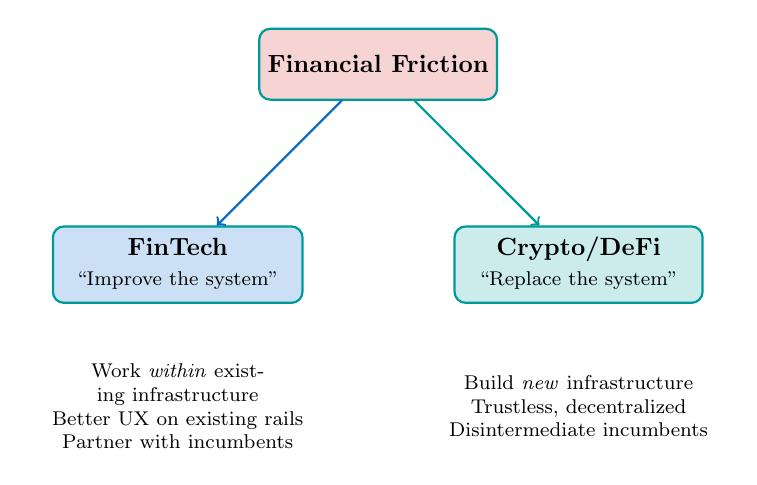
\begin{tikzpicture}[scale=0.9, transform shape]
% Root
\node (friction) [blockchain, minimum width=3cm, fill=dfred!20] {\textbf{Financial Friction}};

% Fork
\node (fintech) [blockchain, below left of=friction, node distance=4cm, minimum width=3.5cm, fill=dfblue!20] {
\begin{tabular}{c}
\textbf{FinTech}\\
\footnotesize ``Improve the system''
\end{tabular}
};

\node (crypto) [blockchain, below right of=friction, node distance=4cm, minimum width=3.5cm, fill=dfteal!20] {
\begin{tabular}{c}
\textbf{Crypto/DeFi}\\
\footnotesize ``Replace the system''
\end{tabular}
};

% Arrows
\draw[->, thick, dfblue] (friction) -- (fintech);
\draw[->, thick, dfteal] (friction) -- (crypto);

% Descriptions
\node[below of=fintech, node distance=2cm, text width=4cm, align=center, font=\footnotesize] {
Work \textit{within} existing infrastructure\\
Better UX on existing rails\\
Partner with incumbents
};

\node[below of=crypto, node distance=2cm, text width=4cm, align=center, font=\footnotesize] {
Build \textit{new} infrastructure\\
Trustless, decentralized\\
Disintermediate incumbents
};
\end{tikzpicture}
\end{center}
\end{frame}

% =====================================================================
% FRAME 6: PHILOSOPHY #1 - FINTECH OVERVIEW
% =====================================================================
\begin{frame}{Philosophy \#1: FinTech}
\begin{center}
\textbf{\Large ``Better UX on Existing Rails''}
\end{center}

\vspace{3mm}
\begin{columns}[T]
\begin{column}{0.5\textwidth}
\textbf{Core Belief:}\\
The existing financial infrastructure works. It just needs:
\begin{itemize}
\item Better user interfaces
\item More efficient processes
\item Smarter technology
\item New business models
\end{itemize}

\vspace{3mm}
\textbf{Key Technologies:}
\begin{itemize}
\item APIs and Open Banking
\item Mobile apps
\item Cloud computing
\item Machine learning
\item Big data analytics
\end{itemize}
\end{column}
\begin{column}{0.47\textwidth}
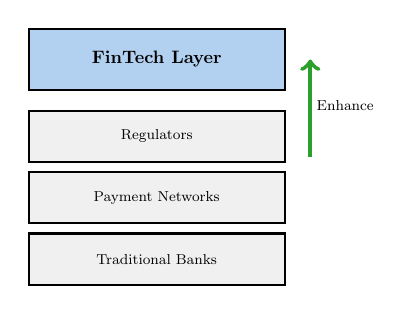
\begin{tikzpicture}[scale=0.65, transform shape]
% Traditional stack with FinTech layer
\draw[thick, fill=lightgray] (0,0) rectangle (5,1);
\node at (2.5,0.5) {\footnotesize Traditional Banks};

\draw[thick, fill=lightgray] (0,1.2) rectangle (5,2.2);
\node at (2.5,1.7) {\footnotesize Payment Networks};

\draw[thick, fill=lightgray] (0,2.4) rectangle (5,3.4);
\node at (2.5,2.9) {\footnotesize Regulators};

% FinTech layer on top
\draw[thick, fill=dfblue!30] (0,3.8) rectangle (5,5);
\node at (2.5,4.4) {\textbf{FinTech Layer}};

% Arrow showing enhancement
\draw[->, ultra thick, dfgreen] (5.5,2.5) -- (5.5,4.4);
\node[right, font=\footnotesize] at (5.5,3.5) {Enhance};
\end{tikzpicture}

\vspace{2mm}
\footnotesize
FinTech builds \textit{on top of} the existing system
\end{column}
\end{columns}
\end{frame}

% =====================================================================
% FRAME 7: FINTECH - TRUST MODEL
% =====================================================================
\begin{frame}{FinTech: The Trust Model}
\begin{center}
\textbf{\Large Institutional Trust}
\end{center}

\vspace{3mm}
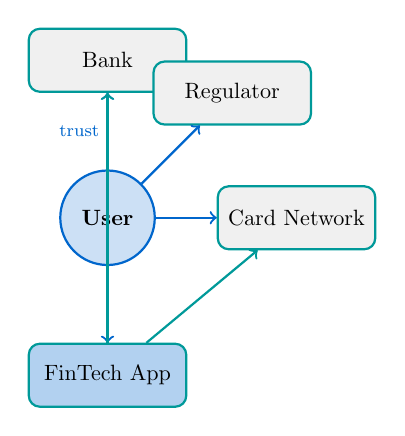
\begin{tikzpicture}[scale=0.8, transform shape]
% User at center
\node (user) [circle, draw=dfblue, thick, fill=dfblue!20, minimum size=1.5cm] at (0,0) {\textbf{User}};

% Institutions around
\node (bank) [blockchain, above of=user, node distance=2.5cm, fill=lightgray] {Bank};
\node (regulator) [blockchain, above right of=user, node distance=2.8cm, fill=lightgray] {Regulator};
\node (card) [blockchain, right of=user, node distance=3cm, fill=lightgray] {Card Network};
\node (fintech) [blockchain, below of=user, node distance=2.5cm, fill=dfblue!30] {FinTech App};

% Trust arrows
\draw[->, thick, dfblue] (user) -- (bank) node[midway, left, font=\footnotesize] {trust};
\draw[->, thick, dfblue] (user) -- (regulator);
\draw[->, thick, dfblue] (user) -- (card);
\draw[->, thick, dfblue] (user) -- (fintech);

% Fintech connects to infrastructure
\draw[->, thick, dfteal] (fintech) -- (bank);
\draw[->, thick, dfteal] (fintech) -- (card);
\end{tikzpicture}

\vspace{3mm}
\begin{block}{How FinTech Trust Works}
\begin{itemize}
\item \textbf{Regulatory oversight} protects consumers
\item \textbf{FDIC insurance} backs deposits
\item \textbf{Chargebacks} reverse fraudulent transactions
\item \textbf{Legal recourse} available through courts
\end{itemize}
\end{block}
\end{frame}

% =====================================================================
% FRAME 8: FINTECH EXAMPLES - PAYMENTS
% =====================================================================
\begin{frame}{FinTech Examples: Payments}
\begin{columns}[T]
\begin{column}{0.48\textwidth}
\textbf{P2P Payments:}
\begin{itemize}
\item \textbf{Venmo} -- Social payments layer on ACH
\item \textbf{Zelle} -- Bank consortium instant transfer
\item \textbf{Cash App} -- P2P + banking features
\end{itemize}

\vspace{3mm}
\textbf{Merchant Payments:}
\begin{itemize}
\item \textbf{Stripe} -- API-first payment processing
\item \textbf{Square} -- POS + ecosystem
\item \textbf{Adyen} -- Global payment platform
\end{itemize}
\end{column}
\begin{column}{0.48\textwidth}
\textbf{Cross-Border:}
\begin{itemize}
\item \textbf{Wise} (TransferWise) -- Mid-market FX rates
\item \textbf{Remitly} -- Remittance focus
\item \textbf{PayPal/Xoom} -- Global reach
\end{itemize}

\vspace{3mm}
\textbf{Common Thread:}\\
\textcolor{dfblue}{All operate on existing payment rails (ACH, SWIFT, card networks) with better interfaces, pricing, and user experience.}
\end{column}
\end{columns}

\vspace{5mm}
\begin{block}{Key Insight}
When you send money via Venmo, it still settles through ACH---FinTech adds a convenience layer, not new infrastructure.
\end{block}
\end{frame}

% =====================================================================
% FRAME 9: FINTECH EXAMPLES - BANKING & LENDING
% =====================================================================
\begin{frame}{FinTech Examples: Banking \& Lending}
\begin{columns}[T]
\begin{column}{0.48\textwidth}
\textbf{Neobanks:}
\begin{itemize}
\item \textbf{Chime} -- No-fee banking via partners
\item \textbf{N26, Revolut} -- European mobile banks
\item \textbf{Nubank} -- Latin America's largest
\item \textbf{Monzo} -- UK challenger bank
\item \textbf{SoFi, Ally} -- Digital-first banking
\end{itemize}

\vspace{3mm}
\textbf{How Neobanks Work:}
\begin{enumerate}
\item Partner with chartered banks
\item Use existing deposit insurance
\item Better UX, lower fees
\item No physical branches
\end{enumerate}
\end{column}
\begin{column}{0.48\textwidth}
\textbf{Digital Lending:}
\begin{itemize}
\item \textbf{LendingClub, Prosper} -- P2P marketplace
\item \textbf{Affirm, Klarna} -- BNPL (Buy Now Pay Later)
\item \textbf{Upstart} -- AI-based underwriting
\item \textbf{Kabbage} -- SMB lending
\end{itemize}

\vspace{3mm}
\textbf{Innovation Approach:}
\begin{itemize}
\item Alternative data for credit decisions
\item Faster approval processes
\item Better user experience
\item \textcolor{dfred}{Still uses traditional credit infrastructure}
\end{itemize}
\end{column}
\end{columns}
\end{frame}

% =====================================================================
% FRAME 10: FINTECH EXAMPLES - INVESTING & INSURANCE
% =====================================================================
\begin{frame}{FinTech Examples: Investing \& Insurance}
\begin{columns}[T]
\begin{column}{0.48\textwidth}
\textbf{Investing/WealthTech:}
\begin{itemize}
\item \textbf{Robinhood} -- Commission-free trading
\item \textbf{Webull} -- Advanced trading features
\item \textbf{Betterment, Wealthfront} -- Robo-advisors
\item \textbf{Acorns, Stash} -- Micro-investing
\item \textbf{Public, M1 Finance} -- Social investing
\end{itemize}

\vspace{3mm}
\textbf{Key Innovation:}\\
Democratized access to investing through lower minimums, no commissions, and simplified UX.
\end{column}
\begin{column}{0.48\textwidth}
\textbf{InsurTech:}
\begin{itemize}
\item \textbf{Lemonade} -- AI-powered claims
\item \textbf{Oscar} -- Health insurance tech
\item \textbf{Root} -- Telematics-based auto
\item \textbf{Hippo} -- Smart home insurance
\item \textbf{Metromile} -- Pay-per-mile auto
\end{itemize}

\vspace{3mm}
\textbf{Key Innovation:}\\
Better risk assessment through data, faster claims processing, improved customer experience.
\end{column}
\end{columns}

\vspace{3mm}
\begin{block}{FinTech Pattern}
\textcolor{dfblue}{Use technology to make existing financial services faster, cheaper, more accessible---without changing the underlying infrastructure.}
\end{block}
\end{frame}

% =====================================================================
% FRAME 11: PHILOSOPHY #2 - CRYPTO/DEFI OVERVIEW
% =====================================================================
\begin{frame}{Philosophy \#2: Crypto/DeFi}
\begin{center}
\textbf{\Large ``New Rails, New Rules''}
\end{center}

\vspace{3mm}
\begin{columns}[T]
\begin{column}{0.5\textwidth}
\textbf{Core Belief:}\\
The existing infrastructure is fundamentally flawed. We need:
\begin{itemize}
\item New trust model (cryptographic, not institutional)
\item Decentralization (no single point of control)
\item Programmable money (smart contracts)
\item Permissionless access
\end{itemize}

\vspace{3mm}
\textbf{Key Technologies:}
\begin{itemize}
\item Blockchain and distributed ledgers
\item Public-key cryptography
\item Consensus mechanisms
\item Smart contracts
\end{itemize}
\end{column}
\begin{column}{0.47\textwidth}
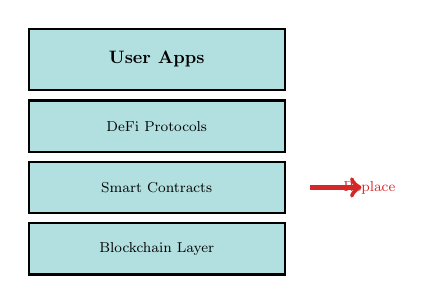
\begin{tikzpicture}[scale=0.65, transform shape]
% Traditional stack (grayed out)
\draw[thick, fill=lightgray, opacity=0.3] (0,0) rectangle (5,1);
\draw[thick, fill=lightgray, opacity=0.3] (0,1.2) rectangle (5,2.2);
\draw[thick, fill=lightgray, opacity=0.3] (0,2.4) rectangle (5,3.4);

% New stack
\draw[thick, fill=dfteal!30] (0,0) rectangle (5,1);
\node at (2.5,0.5) {\footnotesize Blockchain Layer};

\draw[thick, fill=dfteal!30] (0,1.2) rectangle (5,2.2);
\node at (2.5,1.7) {\footnotesize Smart Contracts};

\draw[thick, fill=dfteal!30] (0,2.4) rectangle (5,3.4);
\node at (2.5,2.9) {\footnotesize DeFi Protocols};

\draw[thick, fill=dfteal!30] (0,3.6) rectangle (5,4.8);
\node at (2.5,4.2) {\textbf{User Apps}};

% Arrow showing replacement
\draw[->, ultra thick, dfred] (5.5,1.7) -- node[right, font=\footnotesize] {Replace} (6.5,1.7);
\end{tikzpicture}

\vspace{2mm}
\footnotesize
Crypto/DeFi builds a \textit{parallel} system
\end{column}
\end{columns}
\end{frame}

% =====================================================================
% FRAME 12: CRYPTO/DEFI - TRUST MODEL
% =====================================================================
\begin{frame}{Crypto/DeFi: The Trust Model}
\begin{center}
\textbf{\Large Cryptographic Trust (``Code is Law'')}
\end{center}

\vspace{3mm}
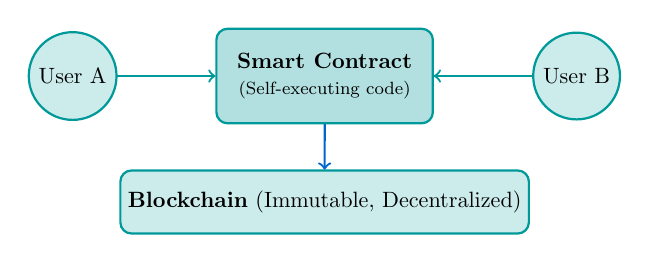
\begin{tikzpicture}[scale=0.8, transform shape]
% User at left
\node (user1) [circle, draw=dfteal, thick, fill=dfteal!20, minimum size=1.2cm] at (0,0) {User A};
\node (user2) [circle, draw=dfteal, thick, fill=dfteal!20, minimum size=1.2cm] at (8,0) {User B};

% Smart contract in center
\node (contract) [blockchain, fill=dfteal!30, minimum width=3cm, minimum height=1.5cm] at (4,0) {
\begin{tabular}{c}
\textbf{Smart Contract}\\
\footnotesize (Self-executing code)
\end{tabular}
};

% Blockchain beneath
\node (blockchain) [blockchain, fill=dfteal!20, minimum width=6cm] at (4,-2) {
\textbf{Blockchain} (Immutable, Decentralized)
};

% Connections
\draw[->, thick, dfteal] (user1) -- (contract);
\draw[->, thick, dfteal] (user2) -- (contract);
\draw[->, thick, dfblue] (contract) -- (blockchain);
\end{tikzpicture}

\vspace{3mm}
\begin{block}{How Crypto/DeFi Trust Works}
\begin{itemize}
\item \textbf{Cryptographic proofs} verify transactions mathematically
\item \textbf{Consensus mechanisms} ensure network agreement
\item \textbf{Smart contracts} execute automatically---no intermediary needed
\item \textbf{Open-source code} is auditable by anyone
\end{itemize}
\end{block}
\end{frame}

% =====================================================================
% FRAME 13: CRYPTO/DEFI EXAMPLES - CURRENCIES & TOKENS
% =====================================================================
\begin{frame}{Crypto/DeFi Examples: Currencies \& Tokens}
\begin{columns}[T]
\begin{column}{0.48\textwidth}
\textbf{Native Cryptocurrencies:}
\begin{itemize}
\item \textbf{Bitcoin (BTC)} -- Digital gold, store of value
\item \textbf{Ethereum (ETH)} -- Smart contract platform
\item \textbf{Solana (SOL)} -- High-speed transactions
\end{itemize}

\vspace{3mm}
\textbf{Stablecoins:}
\begin{itemize}
\item \textbf{USDC} -- Circle, fiat-backed
\item \textbf{USDT} -- Tether, most liquid
\item \textbf{DAI} -- MakerDAO, algorithmic
\item \textbf{FRAX} -- Fractional-algorithmic
\end{itemize}
\end{column}
\begin{column}{0.48\textwidth}
\textbf{Layer 2 Solutions:}
\begin{itemize}
\item \textbf{Polygon} -- Ethereum sidechain
\item \textbf{Arbitrum} -- Optimistic rollups
\item \textbf{Optimism} -- Optimistic rollups
\item \textbf{zkSync} -- Zero-knowledge rollups
\end{itemize}

\vspace{3mm}
\textbf{Purpose:}\\
\textcolor{dfteal}{Create new forms of money and value transfer that operate outside traditional banking infrastructure.}
\end{column}
\end{columns}

\vspace{3mm}
\begin{block}{Key Distinction}
These are not ``better PayPal''---they are entirely new monetary infrastructure with different properties (censorship-resistant, borderless, programmable).
\end{block}
\end{frame}

% =====================================================================
% FRAME 14: CRYPTO/DEFI EXAMPLES - EXCHANGES
% =====================================================================
\begin{frame}{Crypto/DeFi Examples: Exchanges}
\begin{columns}[T]
\begin{column}{0.48\textwidth}
\textbf{Decentralized Exchanges (DEXs):}
\begin{itemize}
\item \textbf{Uniswap} -- Automated Market Maker
\item \textbf{SushiSwap} -- Community fork of Uniswap
\item \textbf{Curve} -- Optimized for stablecoins
\item \textbf{dYdX} -- Decentralized derivatives
\item \textbf{0x Protocol} -- DEX aggregation
\end{itemize}

\vspace{3mm}
\textbf{How DEXs Work:}
\begin{itemize}
\item No central operator
\item Liquidity pools replace order books
\item Smart contracts execute trades
\item Users retain custody of assets
\end{itemize}
\end{column}
\begin{column}{0.48\textwidth}
\textbf{Centralized Exchanges (CEXs):}
\begin{itemize}
\item \textbf{Coinbase} -- US-regulated
\item \textbf{Binance} -- Global, largest volume
\item \textbf{Kraken} -- Security-focused
\end{itemize}

\vspace{2mm}
\footnotesize
\textcolor{dfgray}{Note: CEXs bridge fiat and crypto but operate more like FinTech (custodial, KYC-required)}
\normalsize

\vspace{3mm}
\textbf{Key Contrast:}\\
\textcolor{dfteal}{DEXs are ``pure DeFi'' (permissionless, non-custodial). CEXs are hybrid bridges between worlds.}
\end{column}
\end{columns}
\end{frame}

% =====================================================================
% FRAME 15: CRYPTO/DEFI EXAMPLES - LENDING
% =====================================================================
\begin{frame}{Crypto/DeFi Examples: Lending}
\begin{columns}[T]
\begin{column}{0.48\textwidth}
\textbf{DeFi Lending Protocols:}
\begin{itemize}
\item \textbf{Aave} -- Multi-chain, flash loans
\item \textbf{Compound} -- Algorithmic interest rates
\item \textbf{MakerDAO} -- DAI stablecoin issuance
\item \textbf{Liquity} -- Interest-free borrowing
\end{itemize}

\vspace{3mm}
\textbf{How DeFi Lending Works:}
\begin{enumerate}
\item Deposit collateral to smart contract
\item Borrow against collateral (over-collateralized)
\item Interest rates set algorithmically
\item Liquidation is automatic if under-collateralized
\end{enumerate}
\end{column}
\begin{column}{0.48\textwidth}
\textbf{Comparison to FinTech Lending:}
\renewcommand{\arraystretch}{1.2}
\begin{tabular}{|l|c|c|}
\hline
& \textbf{FinTech} & \textbf{DeFi} \\
\hline
Credit check & Yes & No \\
\hline
Collateral & Optional & Required \\
\hline
Approval & Human/AI & Instant \\
\hline
24/7 access & Limited & Yes \\
\hline
Identity & Required & Anonymous \\
\hline
\end{tabular}

\vspace{3mm}
\textbf{Key Tradeoff:}\\
DeFi: Permissionless but requires collateral\\
FinTech: Credit-based but requires identity
\end{column}
\end{columns}
\end{frame}

% =====================================================================
% FRAME 16: CRYPTO/DEFI EXAMPLES - DERIVATIVES & INFRASTRUCTURE
% =====================================================================
\begin{frame}{Crypto/DeFi Examples: Derivatives \& Infrastructure}
\begin{columns}[T]
\begin{column}{0.48\textwidth}
\textbf{Derivatives Protocols:}
\begin{itemize}
\item \textbf{Synthetix} -- Synthetic assets
\item \textbf{GMX} -- Perpetual futures
\item \textbf{Perp Protocol} -- Virtual AMM derivatives
\item \textbf{Dopex} -- Options protocol
\end{itemize}

\vspace{3mm}
\textbf{What They Enable:}
\begin{itemize}
\item Trade synthetic stocks 24/7
\item Access derivatives without broker
\item Permissionless leverage
\item Global, borderless access
\end{itemize}
\end{column}
\begin{column}{0.48\textwidth}
\textbf{Critical Infrastructure:}
\begin{itemize}
\item \textbf{Chainlink} -- Decentralized oracles
\item \textbf{The Graph} -- Indexing protocol
\item \textbf{IPFS} -- Decentralized storage
\item \textbf{ENS} -- Ethereum naming service
\end{itemize}

\vspace{3mm}
\textbf{Why Infrastructure Matters:}\\
\textcolor{dfteal}{Smart contracts need external data (prices, events). Oracles bridge on-chain and off-chain worlds.}
\end{column}
\end{columns}

\vspace{3mm}
\begin{block}{Common Thread}
All operate on blockchain rails, using smart contracts, without traditional intermediaries.
\end{block}
\end{frame}

% =====================================================================
% FRAME 17: SIDE-BY-SIDE COMPARISON TABLE
% =====================================================================
\begin{frame}{Side-by-Side Comparison}
\begin{center}
\renewcommand{\arraystretch}{1.3}
\begin{tabular}{|l|c|c|}
\hline
\textbf{Dimension} & \textbf{FinTech} & \textbf{Crypto/DeFi} \\
\hline
\textbf{Trust model} & Institutions & Code/Math \\
\hline
\textbf{Infrastructure} & Existing rails & New rails \\
\hline
\textbf{Permission} & Licensed, regulated & Permissionless \\
\hline
\textbf{Identity} & Required (KYC) & Optional (pseudonymous) \\
\hline
\textbf{Reversibility} & Chargebacks possible & Transactions final \\
\hline
\textbf{Speed to market} & Faster (use existing) & Slower (build new) \\
\hline
\textbf{Regulatory clarity} & Higher & Lower \\
\hline
\textbf{User experience} & Polished & Improving \\
\hline
\textbf{Censorship resistance} & Low & High \\
\hline
\end{tabular}
\end{center}
\end{frame}

% =====================================================================
% FRAME 18: DETAILED COMPARISON - TRUST & CUSTODY
% =====================================================================
\begin{frame}{Comparison Deep Dive: Trust \& Custody}
\begin{columns}[T]
\begin{column}{0.48\textwidth}
\textbf{FinTech: Third-Party Custody}
\begin{itemize}
\item Bank holds your deposits
\item Broker holds your securities
\item Insurance protects against failure
\item Legal system enforces rights
\item \textcolor{dfgreen}{\checkmark} Consumer protections
\item \textcolor{dfred}{$\times$} Not your keys, not your coins
\end{itemize}

\vspace{3mm}
\textbf{Implications:}
\begin{itemize}
\item Accounts can be frozen
\item Geographic restrictions apply
\item Dependent on institution solvency
\end{itemize}
\end{column}
\begin{column}{0.48\textwidth}
\textbf{Crypto/DeFi: Self-Custody}
\begin{itemize}
\item Private keys = ownership
\item No counterparty risk (if self-custody)
\item Cannot be seized without keys
\item No geographic boundaries
\item \textcolor{dfgreen}{\checkmark} True ownership
\item \textcolor{dfred}{$\times$} No recovery if keys lost
\end{itemize}

\vspace{3mm}
\textbf{Implications:}
\begin{itemize}
\item Full responsibility on user
\item No customer support
\item Higher technical barrier
\end{itemize}
\end{column}
\end{columns}
\end{frame}

% =====================================================================
% FRAME 19: DETAILED COMPARISON - ACCESS & IDENTITY
% =====================================================================
\begin{frame}{Comparison Deep Dive: Access \& Identity}
\begin{columns}[T]
\begin{column}{0.48\textwidth}
\textbf{FinTech: KYC Required}
\begin{itemize}
\item Government ID verification
\item Address proof required
\item Credit history checked
\item AML/CTF compliance
\end{itemize}

\vspace{3mm}
\textbf{Who Gets Excluded:}
\begin{itemize}
\item Undocumented individuals
\item Those without fixed address
\item Countries under sanctions
\item People with poor credit history
\end{itemize}
\end{column}
\begin{column}{0.48\textwidth}
\textbf{Crypto/DeFi: Permissionless}
\begin{itemize}
\item Only need internet + wallet
\item Pseudonymous by default
\item No credit check
\item No geographic restrictions
\end{itemize}

\vspace{3mm}
\textbf{Who This Serves:}
\begin{itemize}
\item 1.4B unbanked globally
\item Citizens of unstable regimes
\item Privacy-conscious users
\item Cross-border workers
\end{itemize}
\end{column}
\end{columns}

\vspace{3mm}
\begin{block}{The Tradeoff}
\textbf{FinTech:} Protections come with exclusion\\
\textbf{DeFi:} Inclusion comes with fewer protections
\end{block}
\end{frame}

% =====================================================================
% FRAME 20: DETAILED COMPARISON - OPERATIONS
% =====================================================================
\begin{frame}{Comparison Deep Dive: Operating Characteristics}
\begin{center}
\renewcommand{\arraystretch}{1.4}
\begin{tabular}{|l|p{4.5cm}|p{4.5cm}|}
\hline
\textbf{Aspect} & \textbf{FinTech} & \textbf{Crypto/DeFi} \\
\hline
\textbf{Hours} & Business hours, settlement windows, batch processing & 24/7/365 continuous operation \\
\hline
\textbf{Settlement} & T+1 to T+3 days (securities), instant facade (payments) & Minutes to hours (blockchain confirmation) \\
\hline
\textbf{Scalability} & Add servers/databases (proven, costly) & Blockchain trilemma (Layer 2 solutions) \\
\hline
\textbf{Transparency} & Proprietary systems & Open-source, on-chain \\
\hline
\textbf{Composability} & API partnerships (permissioned) & ``Money Legos'' (permissionless) \\
\hline
\end{tabular}
\end{center}
\end{frame}

% =====================================================================
% FRAME 21: TRADEOFFS - FINTECH
% =====================================================================
\begin{frame}{Tradeoffs: FinTech}
\begin{columns}[T]
\begin{column}{0.48\textwidth}
\textbf{Advantages:}
\begin{itemize}
\item[\textcolor{dfgreen}{\checkmark}] Familiar UX
\item[\textcolor{dfgreen}{\checkmark}] Regulatory compliance
\item[\textcolor{dfgreen}{\checkmark}] Consumer protections
\item[\textcolor{dfgreen}{\checkmark}] Fiat integration
\item[\textcolor{dfgreen}{\checkmark}] Customer support
\item[\textcolor{dfgreen}{\checkmark}] Fast iteration
\item[\textcolor{dfgreen}{\checkmark}] Proven business models
\end{itemize}
\end{column}
\begin{column}{0.48\textwidth}
\textbf{Disadvantages:}
\begin{itemize}
\item[\textcolor{dfred}{$\times$}] Still intermediated
\item[\textcolor{dfred}{$\times$}] Geographic restrictions
\item[\textcolor{dfred}{$\times$}] Can be censored/frozen
\item[\textcolor{dfred}{$\times$}] Limited innovation ceiling
\item[\textcolor{dfred}{$\times$}] Data centralization
\item[\textcolor{dfred}{$\times$}] Dependent on banks
\item[\textcolor{dfred}{$\times$}] Exclusion still possible
\end{itemize}
\end{column}
\end{columns}

\vspace{5mm}
\begin{block}{Best For}
Users who want \textbf{better} financial services within the existing system, with familiar protections and convenience.
\end{block}
\end{frame}

% =====================================================================
% FRAME 22: TRADEOFFS - CRYPTO/DEFI
% =====================================================================
\begin{frame}{Tradeoffs: Crypto/DeFi}
\begin{columns}[T]
\begin{column}{0.48\textwidth}
\textbf{Advantages:}
\begin{itemize}
\item[\textcolor{dfgreen}{\checkmark}] Permissionless access
\item[\textcolor{dfgreen}{\checkmark}] Censorship resistant
\item[\textcolor{dfgreen}{\checkmark}] Transparent (open-source)
\item[\textcolor{dfgreen}{\checkmark}] Composable (``money legos'')
\item[\textcolor{dfgreen}{\checkmark}] 24/7 global operation
\item[\textcolor{dfgreen}{\checkmark}] Self-custody possible
\item[\textcolor{dfgreen}{\checkmark}] Programmable money
\end{itemize}
\end{column}
\begin{column}{0.48\textwidth}
\textbf{Disadvantages:}
\begin{itemize}
\item[\textcolor{dfred}{$\times$}] Complex UX
\item[\textcolor{dfred}{$\times$}] Regulatory uncertainty
\item[\textcolor{dfred}{$\times$}] No chargebacks
\item[\textcolor{dfred}{$\times$}] Smart contract risks
\item[\textcolor{dfred}{$\times$}] Volatility (non-stablecoins)
\item[\textcolor{dfred}{$\times$}] Scalability challenges
\item[\textcolor{dfred}{$\times$}] ``Code is law'' rigidity
\end{itemize}
\end{column}
\end{columns}

\vspace{5mm}
\begin{block}{Best For}
Users who need \textbf{different} financial infrastructure---global access, self-sovereignty, censorship resistance, or programmable finance.
\end{block}
\end{frame}

% =====================================================================
% FRAME 23: RISK COMPARISON
% =====================================================================
\begin{frame}{Risk Comparison}
\begin{center}
\renewcommand{\arraystretch}{1.4}
\begin{tabular}{|l|c|c|}
\hline
\textbf{Risk Type} & \textbf{FinTech} & \textbf{Crypto/DeFi} \\
\hline
\textbf{Counterparty Risk} & Medium (institutional) & Low (if self-custody) \\
\hline
\textbf{Smart Contract Risk} & N/A & High (bugs, exploits) \\
\hline
\textbf{Regulatory Risk} & Low (compliant) & High (uncertain) \\
\hline
\textbf{Custodial Risk} & Medium (FDIC helps) & High (lost keys = lost funds) \\
\hline
\textbf{Censorship Risk} & Medium (can be frozen) & Low (resistant) \\
\hline
\textbf{Volatility Risk} & Low (fiat-based) & High (crypto) / Low (stables) \\
\hline
\textbf{Recovery Options} & High (legal recourse) & Low (irreversible) \\
\hline
\end{tabular}
\end{center}

\vspace{3mm}
\textbf{Key Insight:} Neither approach eliminates risk---they trade one set of risks for another.
\end{frame}

% =====================================================================
% FRAME 24: THE CONVERGENCE
% =====================================================================
\begin{frame}{The Convergence}
\begin{center}
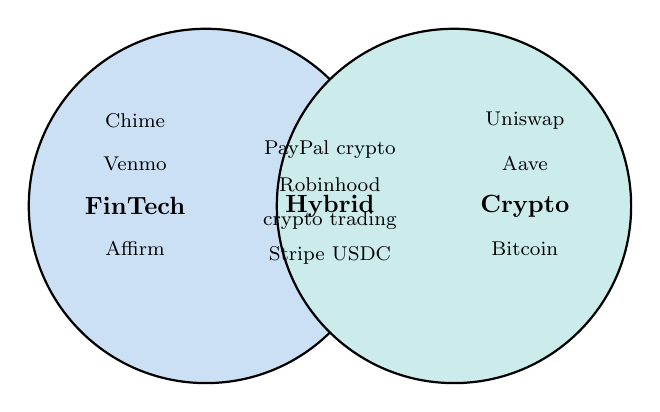
\begin{tikzpicture}[scale=0.9, transform shape]
% Two circles overlapping
\draw[thick, fill=dfblue!20] (0,0) circle (2.5cm);
\draw[thick, fill=dfteal!20] (3.5,0) circle (2.5cm);

% Labels
\node at (-1,0) {\textbf{FinTech}};
\node at (4.5,0) {\textbf{Crypto}};
\node at (1.75,0) {\textbf{Hybrid}};

% Examples in overlap
\node[font=\footnotesize] at (1.75,0.8) {PayPal crypto};
\node[font=\footnotesize] at (1.75,0.3) {Robinhood};
\node[font=\footnotesize] at (1.75,-0.2) {crypto trading};
\node[font=\footnotesize] at (1.75,-0.7) {Stripe USDC};

% Pure examples
\node[font=\footnotesize] at (-1,1.2) {Chime};
\node[font=\footnotesize] at (-1,0.6) {Venmo};
\node[font=\footnotesize] at (-1,-0.6) {Affirm};

\node[font=\footnotesize] at (4.5,1.2) {Uniswap};
\node[font=\footnotesize] at (4.5,0.6) {Aave};
\node[font=\footnotesize] at (4.5,-0.6) {Bitcoin};
\end{tikzpicture}
\end{center}

\vspace{3mm}
\textbf{Increasingly:}
\begin{itemize}
\item FinTech companies add crypto features (PayPal, Revolut)
\item Crypto projects improve UX toward FinTech standards
\item Traditional banks explore blockchain settlement
\item Lines blur, but \textbf{philosophies remain distinct}
\end{itemize}
\end{frame}

% =====================================================================
% FRAME 25: CONVERGENCE EXAMPLES
% =====================================================================
\begin{frame}{Convergence in Practice}
\begin{columns}[T]
\begin{column}{0.48\textwidth}
\textbf{FinTech Adding Crypto:}
\begin{itemize}
\item \textbf{PayPal} -- Buy/sell/hold crypto
\item \textbf{Robinhood} -- Crypto trading alongside stocks
\item \textbf{Stripe} -- USDC payouts for merchants
\item \textbf{Visa/Mastercard} -- Crypto card programs
\item \textbf{Block (Square)} -- Bitcoin integration
\end{itemize}

\vspace{3mm}
\textbf{Why?}\\
Customer demand, new revenue streams, competitive positioning
\end{column}
\begin{column}{0.48\textwidth}
\textbf{Crypto Improving UX:}
\begin{itemize}
\item \textbf{Account abstraction} -- No gas fees for users
\item \textbf{Social recovery} -- Not losing keys forever
\item \textbf{Fiat on-ramps} -- Easy entry points
\item \textbf{Mobile-first wallets} -- Better interfaces
\item \textbf{L2 solutions} -- Lower costs, faster speeds
\end{itemize}

\vspace{3mm}
\textbf{Why?}\\
Mass adoption requires FinTech-level UX
\end{column}
\end{columns}

\vspace{3mm}
\begin{block}{The Question}
Will convergence produce the ``best of both worlds''---or compromise the unique benefits of each?
\end{block}
\end{frame}

% =====================================================================
% FRAME 26: CLASSIFICATION FRAMEWORK
% =====================================================================
\begin{frame}{Classification Framework}
\textbf{How to classify any financial innovation:}

\vspace{3mm}
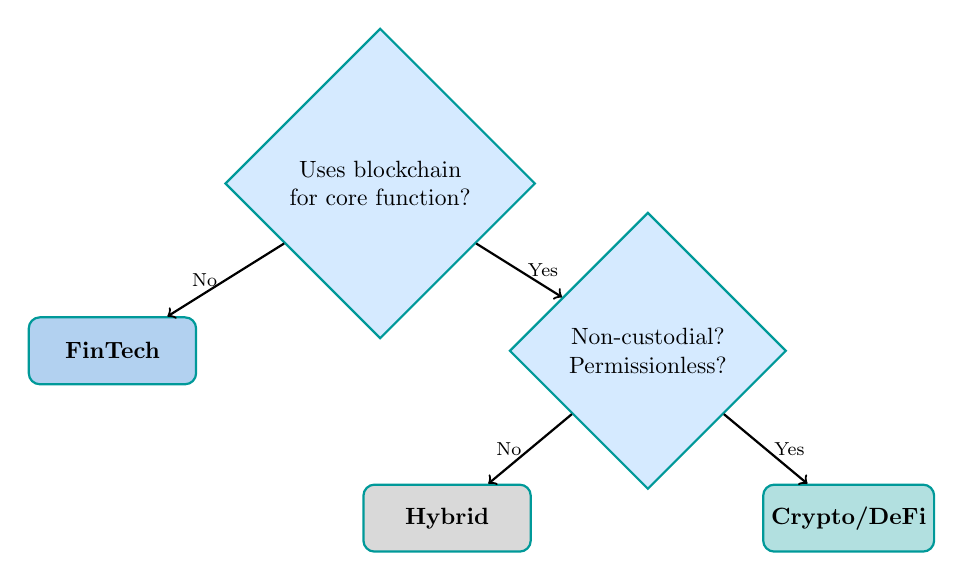
\begin{tikzpicture}[scale=0.85, transform shape]
% Decision tree
\node (q1) [decision, minimum width=1cm, text width=3.5cm] at (0,0) {Uses blockchain for core function?};

\node (fintech) [blockchain, fill=dfblue!30] at (-4,-2.5) {\textbf{FinTech}};
\node (q2) [decision, minimum width=1cm, text width=3cm] at (4,-2.5) {Non-custodial? Permissionless?};

\node (hybrid) [blockchain, fill=dfgray!30] at (1,-5) {\textbf{Hybrid}};
\node (defi) [blockchain, fill=dfteal!30] at (7,-5) {\textbf{Crypto/DeFi}};

\draw[->, thick] (q1) -- node[left, font=\footnotesize] {No} (fintech);
\draw[->, thick] (q1) -- node[right, font=\footnotesize] {Yes} (q2);
\draw[->, thick] (q2) -- node[left, font=\footnotesize] {No} (hybrid);
\draw[->, thick] (q2) -- node[right, font=\footnotesize] {Yes} (defi);
\end{tikzpicture}

\vspace{3mm}
\footnotesize
\textbf{Examples:}\\
Venmo (No blockchain) $\rightarrow$ FinTech | Coinbase (Blockchain, custodial) $\rightarrow$ Hybrid | Uniswap (Blockchain, non-custodial) $\rightarrow$ DeFi
\end{frame}

% =====================================================================
% FRAME 27: CLASSIFICATION EXERCISE
% =====================================================================
\begin{frame}{Classification Exercise}
\textbf{For each innovation, decide: FinTech or Crypto/DeFi?}

\vspace{3mm}
\begin{enumerate}
\item A mobile app that rounds up purchases and invests the change in ETFs
\pause
\textcolor{dfblue}{\textbf{FinTech}} (uses traditional brokerage)
\pause
\item A protocol that lets you earn interest by lending stablecoins
\pause
\textcolor{dfteal}{\textbf{Crypto/DeFi}} (smart contracts, no intermediary)
\pause
\item A bank that has no physical branches and only mobile apps
\pause
\textcolor{dfblue}{\textbf{FinTech}} (still a licensed bank, uses ACH)
\pause
\item A system where you can trade tokenized stocks 24/7
\pause
\textcolor{dfteal}{\textbf{Crypto/DeFi}} (synthetic assets, blockchain settlement)
\pause
\item A service that uses AI to approve loans faster
\pause
\textcolor{dfblue}{\textbf{FinTech}} (better process, same infrastructure)
\end{enumerate}
\end{frame}

% =====================================================================
% FRAME 28: REAL-WORLD USE CASES
% =====================================================================
\begin{frame}{Real-World Use Cases: When to Choose Which?}
\begin{columns}[T]
\begin{column}{0.48\textwidth}
\textbf{Choose FinTech When:}
\begin{itemize}
\item You want consumer protections
\item Regulatory compliance is required
\item You need customer support
\item Working within a stable banking system
\item Fiat currency is primary
\item Business-to-business with contracts
\end{itemize}

\vspace{2mm}
\textbf{Examples:}
\begin{itemize}
\item Payroll processing
\item Mortgage applications
\item Business expense management
\item Retail investing
\end{itemize}
\end{column}
\begin{column}{0.48\textwidth}
\textbf{Choose Crypto/DeFi When:}
\begin{itemize}
\item Permissionless access is essential
\item Cross-border without intermediaries
\item 24/7 operation is critical
\item Programmable money is needed
\item Censorship resistance matters
\item Self-custody is preferred
\end{itemize}

\vspace{2mm}
\textbf{Examples:}
\begin{itemize}
\item International remittances (high-fee corridors)
\item Savings in unstable currency regimes
\item DAO treasury management
\item Permissionless derivatives access
\end{itemize}
\end{column}
\end{columns}
\end{frame}

% =====================================================================
% FRAME 29: DISCUSSION - TEAM DEBATE
% =====================================================================
\begin{frame}{Discussion: Which Philosophy Do You Prefer?}
\begin{columns}[T]
\begin{column}{0.48\textwidth}
\textbf{Team FinTech argues:}
\begin{itemize}
\item ``If it ain't broke, don't rebuild it''
\item Regulatory protection matters
\item Most users want convenience, not sovereignty
\item Crypto is too volatile and risky
\item The existing system has centuries of evolution
\end{itemize}
\end{column}
\begin{column}{0.48\textwidth}
\textbf{Team Crypto argues:}
\begin{itemize}
\item ``The system IS broke for billions''
\item Financial freedom requires autonomy
\item Permissionless access is a human right
\item Code is more trustworthy than institutions
\item Innovation requires new foundations
\end{itemize}
\end{column}
\end{columns}

\vspace{5mm}
\begin{block}{Discussion Questions}
\begin{itemize}
\item Is there room for both philosophies to coexist?
\item Under what circumstances would you choose each?
\item What would make you switch from one to the other?
\end{itemize}
\end{block}
\end{frame}

% =====================================================================
% FRAME 30: APPLICATION - SCENARIO ANALYSIS
% =====================================================================
\begin{frame}{Application: Scenario Analysis}
\textbf{For each scenario, which approach is better suited?}

\vspace{3mm}
\begin{enumerate}
\item \textbf{A freelancer in Argentina} needs to receive USD payments from US clients while the peso devalues rapidly.
\vspace{1mm}
\begin{itemize}
\item[\textcolor{dfteal}{$\rightarrow$}] \textbf{DeFi:} Stablecoin payments avoid forex restrictions, instant settlement
\end{itemize}

\vspace{2mm}
\item \textbf{A US retiree} wants to set up automatic monthly investments in index funds.
\vspace{1mm}
\begin{itemize}
\item[\textcolor{dfblue}{$\rightarrow$}] \textbf{FinTech:} Robinhood/Betterment offers familiar UX, tax-advantaged accounts
\end{itemize}

\vspace{2mm}
\item \textbf{A DAO} needs to manage a treasury across global contributors without a legal entity.
\vspace{1mm}
\begin{itemize}
\item[\textcolor{dfteal}{$\rightarrow$}] \textbf{DeFi:} Multisig wallets, on-chain governance, no jurisdiction issues
\end{itemize}

\vspace{2mm}
\item \textbf{A small business} needs a line of credit and expense management.
\vspace{1mm}
\begin{itemize}
\item[\textcolor{dfblue}{$\rightarrow$}] \textbf{FinTech:} Brex/Ramp offers credit, integrations, customer support
\end{itemize}
\end{enumerate}
\end{frame}

% =====================================================================
% FRAME 31: EXECUTIVE SUMMARY
% =====================================================================
\begin{frame}{Executive Summary}
\begin{block}{The Fundamental Fork}
Both FinTech and Crypto/DeFi target the same financial frictions but approach them fundamentally differently.
\end{block}

\vspace{3mm}
\textbf{Key Takeaways:}
\begin{enumerate}
\item \textbf{FinTech = ``Improve the system''} -- Better UX on existing rails, works with regulators and banks, institutional trust model

\vspace{2mm}
\item \textbf{Crypto/DeFi = ``Replace the system''} -- New rails, permissionless, cryptographic trust, disintermediates incumbents

\vspace{2mm}
\item \textbf{Neither is universally better} -- Choose based on use case, risk tolerance, and values

\vspace{2mm}
\item \textbf{Convergence is happening} -- But the philosophical divide remains meaningful

\vspace{2mm}
\item \textbf{Classification skill is essential} -- Understand whether an innovation improves or replaces infrastructure
\end{enumerate}
\end{frame}

% =====================================================================
% FRAME 32: CONCEPT MAP
% =====================================================================
\begin{frame}{Concept Map: The Philosophical Fork}
\begin{center}
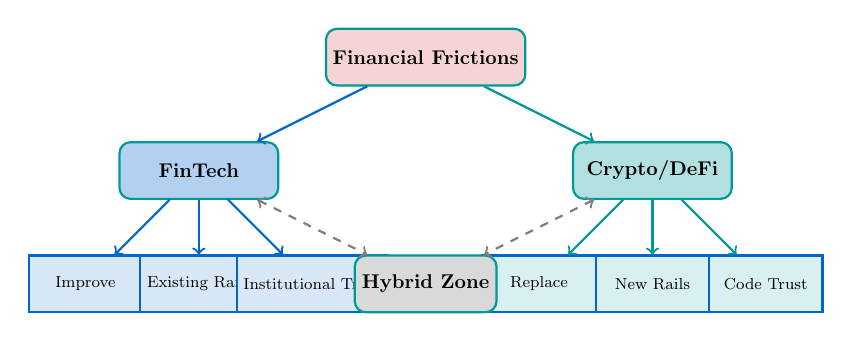
\begin{tikzpicture}[scale=0.72, transform shape]
% Central concept
\node (friction) [blockchain, fill=dfred!20, minimum width=3.5cm] at (6,5) {\textbf{Financial Frictions}};

% Fork
\node (fintech) [blockchain, fill=dfblue!30, minimum width=2.8cm] at (2,3) {\textbf{FinTech}};
\node (crypto) [blockchain, fill=dfteal!30, minimum width=2.8cm] at (10,3) {\textbf{Crypto/DeFi}};

% FinTech properties
\node (improve) [process, fill=dfblue!15, minimum width=2cm, font=\footnotesize] at (0,1) {Improve};
\node (existing) [process, fill=dfblue!15, minimum width=2cm, font=\footnotesize] at (2,1) {Existing Rails};
\node (inst) [process, fill=dfblue!15, minimum width=2cm, font=\footnotesize] at (4,1) {Institutional Trust};

% Crypto properties
\node (replace) [process, fill=dfteal!15, minimum width=2cm, font=\footnotesize] at (8,1) {Replace};
\node (new) [process, fill=dfteal!15, minimum width=2cm, font=\footnotesize] at (10,1) {New Rails};
\node (code) [process, fill=dfteal!15, minimum width=2cm, font=\footnotesize] at (12,1) {Code Trust};

% Convergence
\node (hybrid) [blockchain, fill=dfgray!30, minimum width=2.5cm] at (6,1) {\textbf{Hybrid Zone}};

% Connections
\draw[->, thick, dfblue] (friction) -- (fintech);
\draw[->, thick, dfteal] (friction) -- (crypto);

\draw[->, thick, dfblue] (fintech) -- (improve);
\draw[->, thick, dfblue] (fintech) -- (existing);
\draw[->, thick, dfblue] (fintech) -- (inst);

\draw[->, thick, dfteal] (crypto) -- (replace);
\draw[->, thick, dfteal] (crypto) -- (new);
\draw[->, thick, dfteal] (crypto) -- (code);

\draw[<->, thick, dashed, dfgray] (fintech) -- (hybrid);
\draw[<->, thick, dashed, dfgray] (crypto) -- (hybrid);
\end{tikzpicture}
\end{center}

\vspace{2mm}
\footnotesize
\textbf{Reading the map:} Both philosophies emerge from the same frictions but diverge in approach. The hybrid zone represents the growing convergence.
\end{frame}

% =====================================================================
% FRAME 33: KEY TERMS & DEFINITIONS (1/2)
% =====================================================================
\begin{frame}{Key Terms \& Definitions (1/2)}
\begin{description}
\item[FinTech] Financial technology that improves existing financial infrastructure through better UX, processes, and technology while working within traditional systems.

\vspace{2mm}
\item[Crypto/DeFi] Decentralized finance built on blockchain infrastructure that aims to replace traditional intermediaries with trustless, permissionless protocols.

\vspace{2mm}
\item[Institutional Trust] Trust model based on regulated institutions, legal contracts, and government oversight (banks, regulators, courts).

\vspace{2mm}
\item[Cryptographic Trust] Trust model based on mathematical proofs, consensus mechanisms, and immutable code (``code is law'').

\vspace{2mm}
\item[Permissionless] Systems that anyone can access without approval from a central authority (no KYC, no geographic restrictions).

\vspace{2mm}
\item[Self-Custody] Holding assets under your own control via private keys, without third-party intermediaries.
\end{description}
\end{frame}

% =====================================================================
% FRAME 34: KEY TERMS & DEFINITIONS (2/2)
% =====================================================================
\begin{frame}{Key Terms \& Definitions (2/2)}
\begin{description}
\item[KYC (Know Your Customer)] Regulatory requirement to verify customer identity---standard in FinTech, often absent in pure DeFi.

\vspace{2mm}
\item[Smart Contract] Self-executing code on blockchain that automatically enforces agreement terms without intermediaries.

\vspace{2mm}
\item[Composability] ``Money Legos''---ability to combine DeFi protocols permissionlessly to create new financial products.

\vspace{2mm}
\item[Censorship Resistance] Property of systems where no single party can block or reverse transactions.

\vspace{2mm}
\item[Neobank] Digital-only bank without physical branches, typically a FinTech that partners with licensed banks.

\vspace{2mm}
\item[DEX (Decentralized Exchange)] Exchange protocol running on smart contracts without central operator or custody.

\vspace{2mm}
\item[Oracle] Service that provides external (off-chain) data to smart contracts (e.g., Chainlink for price feeds).
\end{description}
\end{frame}

% =====================================================================
% FRAME 35: COMMON MISCONCEPTIONS
% =====================================================================
\begin{frame}{Common Misconceptions}
\begin{enumerate}
\item \textbf{``All crypto companies are DeFi''}\\
\textcolor{dfred}{FALSE:} Centralized exchanges like Coinbase operate more like FinTech (custodial, KYC-required). Pure DeFi is permissionless and non-custodial.

\vspace{3mm}
\item \textbf{``FinTech is not innovative because it uses old rails''}\\
\textcolor{dfred}{FALSE:} Innovation in UX, business models, and accessibility can be transformative even on existing infrastructure. Stripe revolutionized payments without changing the underlying rails.

\vspace{3mm}
\item \textbf{``DeFi is only for speculation and crypto gambling''}\\
\textcolor{dfred}{FALSE:} While speculation exists, DeFi also enables real use cases: remittances, savings in unstable currencies, permissionless lending, and programmable finance.

\vspace{3mm}
\item \textbf{``The two philosophies cannot coexist''}\\
\textcolor{dfred}{FALSE:} They serve different needs and user preferences. The convergence zone shows productive overlap, and users can choose based on specific requirements.
\end{enumerate}
\end{frame}

% =====================================================================
% FRAME 36: SELF-ASSESSMENT QUESTION 1
% =====================================================================
\begin{frame}{Self-Assessment Question 1}
\textbf{Question:} What is the core philosophy of FinTech?

\vspace{5mm}
\begin{enumerate}[A)]
\item Replace the existing financial system with blockchain
\item Improve the existing financial system with better UX and technology
\item Eliminate all financial intermediaries
\item Create permissionless financial infrastructure
\end{enumerate}

\vspace{5mm}
\pause
\textbf{Answer: B}

\vspace{3mm}
\textbf{Explanation:} FinTech's core belief is that the existing financial infrastructure works but needs better user interfaces, more efficient processes, and smarter technology. It builds on top of existing rails rather than replacing them.
\end{frame}

% =====================================================================
% FRAME 37: SELF-ASSESSMENT QUESTIONS 2-3
% =====================================================================
\begin{frame}{Self-Assessment Questions 2-3}
\textbf{Question 2:} What is the identity verification difference between FinTech and Crypto/DeFi?

\vspace{2mm}
\begin{enumerate}[A)]
\item FinTech requires KYC verification; Crypto/DeFi systems can be pseudonymous
\item Both require full identity verification
\item Crypto/DeFi requires more identity verification than FinTech
\item Neither requires any form of identity verification
\end{enumerate}

\pause
\textbf{Answer: A} -- FinTech operates within regulatory frameworks requiring KYC. Crypto/DeFi can operate pseudonymously with wallet addresses.

\vspace{5mm}
\textbf{Question 3:} What is the fundamental fork that distinguishes FinTech from Crypto/DeFi?

\vspace{2mm}
\begin{enumerate}[A)]
\item Mobile-first vs. desktop-first design
\item Improve the existing system vs. replace the system
\item B2B vs. B2C business models
\item Domestic vs. international focus
\end{enumerate}

\pause
\textbf{Answer: B} -- The fundamental fork is philosophical: FinTech improves existing infrastructure; Crypto/DeFi aims to replace it with new trustless, decentralized infrastructure.
\end{frame}

% =====================================================================
% FRAME 38: WHAT'S NEXT
% =====================================================================
\begin{frame}{What's Next: Topic 1.4 -- Landscape Overview}
\begin{block}{Preview}
Now that you understand the two philosophical approaches, we will map the \textbf{entire digital finance landscape} to see how these innovations fit together.
\end{block}

\vspace{3mm}
\textbf{Topics in 1.4:}
\begin{itemize}
\item The six sectors of digital finance: Payments, Lending, Trading, Banking, Insurance, Investing
\item Infrastructure layers: Blockchain, APIs, Data, Identity
\item How FinTech and Crypto/DeFi examples map across sectors
\item Connections and dependencies between sectors
\item Locating any innovation within the landscape
\end{itemize}

\vspace{3mm}
\textbf{Key Question:}
\begin{center}
\textit{``Where does any given innovation fit in the broader map of digital finance?''}
\end{center}
\end{frame}

% =====================================================================
% FRAME 39: RESOURCES
% =====================================================================
\begin{frame}{Resources for Further Learning}
\textbf{Books:}
\begin{itemize}
\item \textit{The FinTech Book} -- Chishti \& Barberis (2016)
\item \textit{DeFi and the Future of Finance} -- Campbell Harvey et al. (2021)
\item \textit{The Infinite Machine} -- Camila Russo (Ethereum history)
\end{itemize}

\vspace{3mm}
\textbf{Online Resources:}
\begin{itemize}
\item DeFi Llama (\url{defillama.com}) -- DeFi protocol analytics
\item CB Insights FinTech reports -- Industry analysis
\item Bankless podcast -- DeFi-focused content
\item a]6z Crypto Startup School -- Free curriculum
\end{itemize}

\vspace{3mm}
\textbf{Research:}
\begin{itemize}
\item BIS Working Papers on FinTech
\item Federal Reserve FinTech reports
\item Academic journals: \textit{Journal of Financial Economics}, \textit{Review of Financial Studies}
\end{itemize}
\end{frame}

% =====================================================================
% FRAME 40: QUESTIONS
% =====================================================================
\begin{frame}{Questions?}
\begin{center}
\vspace{1cm}
{\Large \textbf{Topic 1.3: FinTech vs. Crypto/DeFi}}

\vspace{1cm}
\textbf{Key Takeaway:}\\
\textit{``Same frictions, different philosophies---\\improve the system or replace it?''}

\vspace{1.5cm}
\textbf{Contact:}\\
Joerg Osterrieder\\
\texttt{joerg.osterrieder@hm.edu}

\vspace{1cm}
{\small Next: Topic 1.4 -- Landscape Overview}
\end{center}
\end{frame}

\end{document}
